\section{KLR iYangians}
\label{klrtY}
Recall the quiver with involution from \cref{sec:qwi}. 
Throughout this section we let $\lambda=\sum_{i\in Q_0}\lambda_i \varpi_i$ be a dominant weight, ${}^\tau \lambda=\lambda+\tau \lambda$, $\mu$ be a $\tau$-invariant weight such that ${}^\tau\lambda \geq \mu$. We also fix a set of parameters $\bR=(\bR_i)_{i\in Q_0}\in \prod_{i\in Q_0} \C^{\lambda_i}$ so that each $\bR_i$ is of size $\lambda_i$.%, and let $\bR$ be a set of parameters $\bR$ of weight $\lambda$. 
%\red{fix some orientation for the quiver}

\subsection{Shifted iYangian}
 Recall the symmetric generalized Cartan matrix $C$ from \cref{sec:KLR} and the symmetric Kac-Moody algebra $\mathfrak{g}$. Following \cite[Def. 3.1]{SSX25} (see also \cite{LWW,LWW2}), we now define the shifted iYangian ${}^{\tau}\mathbf{Y}_{\mu}(\mathfrak{g})$ . 
\begin{definition}
\label{shiftedTY}
The shifted iYangian ${}^{\tau}\mathbf{Y}_{\mu}(\mathfrak{g})$ is the $\mathbb{C}(\hbar)$-algebra generated by 
$h_{i,r}$ and $b_{i,s}$ for $i\in Q_0, r\geq -( \alpha_i,\mu)-1$ and $s\geq 0$, subject to the following relations:
\begin{align}
\label{eq:hcomm}
    & {\left[h_{i, r}, h_{j, s}\right]=0, \qquad 
    h_{i,s} = (-1)^{s+1} h_{\tau i,s}}, 
        % &(r,s\in \mathbb{Z})
        \\
\label{eq:hbcomm}
    & {\left[h_{i, r+2}, b_{j, s}\right]-\left[h_{i, r}, b_{j, s+2}\right]} 
    =\frac{c_{i j}-c_{\tau i, j}}{2} \hbar\left\{h_{i, r+1}, b_{j, s}\right\}
    \\\notag  & \qquad 
    +\frac{c_{i j}+c_{\tau i, j}}{2} \hbar\left\{h_{i, r}, b_{j, s+1}\right\}
    +\frac{c_{i j} c_{\tau i, j}}{4} \hbar^2\left[h_{i, r}, b_{j, s}\right], 
        % &(r\in \mathbb{Z},s\geq0)
        \\
\label{eq:bcomm}
    & {\left[b_{i, r+1}, b_{j, s}\right]-\left[b_{i, r}, b_{j, s+1}\right]=\frac{c_{i j}}{2}\hbar \left\{b_{i, r}, b_{j, s}\right\}-2 \delta_{\tau i, j}(-1)^r h_{j, r+s+1}},
        % &(r,s\geq 0)
\end{align}
and the Serre-type relations  
\begin{itemize}
    \item when $c_{i j}=0$, we have %commutative Serre relations
\begin{equation}\label{eq:commSerre}
    \left[b_{i, r}, b_{j, s}\right]=\delta_{\tau i, j}(-1)^r h_{j, r+s};
\end{equation}
\item when $c_{i j}=-1, j \neq \tau i \neq i$, we have %usual Serre relations
\begin{equation}\label{eq:usualSerre}
    \operatorname{Sym}_{k_1, k_2}\left[b_{i, k_1},\left[b_{i, k_2}, b_{j, r}\right]\right]=0;
\end{equation}
\item when $c_{i, \tau i}=-1$, we have 
\begin{equation}\label{eq:iSerre}
    \operatorname{Sym}_{k_1, k_2}\left[b_{i, k_1},\left[b_{i, k_2}, b_{\tau i, r}\right]\right]=\frac{4}{3} \operatorname{Sym}_{k_1, k_2}(-1)^{k_1} \sum_{p=0}^{\infty} 3^{-p}\left[b_{i, k_2+p}, h_{\tau i, k_1+r-p}\right].
\end{equation}
\end{itemize}
Here we have adopted the convention that 
\begin{equation}\label{eq:vanishing}
\mbox{$h_{i,r}=0$ if $r<-(\alpha_i, \mu)-1$ and $h_{i,r}=\zeta_i$ if $r=-(\alpha_i, \mu)-1$},
\end{equation}
where $\zeta$ is a family of parameters 
$\zeta = (\zeta_i)_{i \in Q_0} \in \bigl(\mathbb{C}(\hbar)^\times\bigr)^I$ satisfying 
\begin{equation}\label{eq:zeta}
  \zeta_i = (-1)^{(\alpha_i, \mu)}\,\zeta_{\tau(i)} 
   \in \mathbb{C}(\hbar)^\times.
\end{equation}
\end{definition}
We note that the right-hand side of \cref{eq:iSerre} is a finite sum by the convention \cref{eq:vanishing}. By \cite[Rem 3.3]{SSX25}, the shifted iYangian ${}^{\tau}\mathbf{Y}_{\mu}(\mathfrak{g})$ is independent of the choice of $\zeta$ up to an algebra automorphism. We then define the following generating functions
\begin{align}
\label{generatingfunction}
h_i(z) & = \hbar\sum_{r\in \mathbb{Z}}h_{i,r}z^{-r-1},&
h_i^\circ(z) & = \hbar\sum_{r\geq 0}h_{i,r}z^{-r-1},&
b_i(z) & = \hbar\sum_{s\geq 0}b_{i,s}z^{-s-1}.
\end{align}


\subsection{iGKLO representations}
\label{sec:iGKLO}
Suppose that ${}^\tau\lambda-\mu=\sum_{i\in Q_0} v_i \alpha_i$ with $v_i=v_{\tau i}\geq 0$. 
Similar to \cite[Sect. 2.1]{KTWWY19}, we fix a parity bipartition $$Q_0=Q_0^{(+)}\sqcup Q_0^{(-)}$$ and  we
call vertices in $Q_0^{(+)}$ {\bf even} and those in $ Q_0^{(-)}$
{\bf odd}. We orient $\Qui$ so that edges of $\Qui$ always point from even vertices to odd ones. Thus we have 
\[
\tau (Q_0^{(\pm)})=Q_0^{(\mp)}.
\]
We then fix any total order on $Q_0^{(+)}$. This also determines a total order on $Q_0^{(-)}$ such that $i<j$ if and only if $\tau i > \tau j$ for any $i,j\in Q_0^{(-)}$.

\begin{remark}
    We note that, the results in this section does not depend on the total order we choose on $Q_0^{(+)}$, unlike \cite[Sect. 2.1]{KTWWY19} which assumes the even indices come before the odd ones. The key point for us is that, by our assumption, there is no arrow between any two even vertices.
\end{remark}

\begin{example}[Type AIII]
    Consider a quiver with involution obtained from a Satake diagram of type AIII (see \cite{Ara62}) as follows:
    \[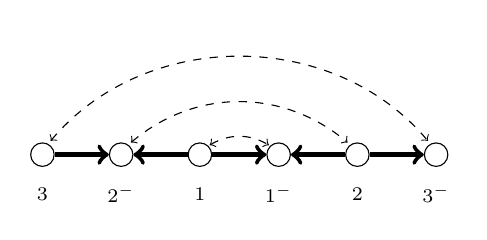
\begin{tikzpicture}[scale=1, 
                    arrow/.style={<->,dashed}]
\foreach \i in {0,...,5}
    \node[circle, draw, inner sep=3pt] (a\i) at (\i,0) {};
    \foreach \i in {0,...,5}
    \node (b\i) at (\i,.05) {};
    \node  at (0,-.5) {$\scriptstyle 3$};
    \node  at (1,-.5) {$\scriptstyle 2^-$};
    \node  at (2,-.5) {$\scriptstyle 1$};
    \node  at (3,-.5) {$\scriptstyle 1^-$};
    \node  at (4,-.5) {$\scriptstyle 2$};
    \node  at (5,-.5) {$\scriptstyle 3^-$};
\draw[arrow] (b0) to[bend left=50] (b5);
\draw[arrow] (b1) to[bend left=40] (b4);
\draw[arrow] (b2) to[bend left=30] (b3);
\draw[->,ultra thick] (a0) -- (a1); 
\draw[->,ultra thick] (a2) -- (a1); 
\draw[->,ultra thick] (a2) -- (a3); 
\draw[->,ultra thick] (a4) -- (a3); 
\draw[->,ultra thick] (a4) -- (a5); 
\end{tikzpicture}
\]
where $\tau$ is indicated by the dashed arrows. We can choose \[
Q_0^{(+)}=\{1,2,3\},\quad Q_0^{(-)}=\{1^-,2^-,3^-\}.
\]
The total order on $Q_0^{(+)}$ can be chosen as $1<2<3$, then the corresponding total order on $Q_0^{(-)}$ is $3^-<2^-<1^-$.
\end{example}

 Consider the polynomial ring
$$ P = \C[\hbar][x_{i,j} : i \in Q_0^{(+)}, 1 \leqslant j \leqslant v_i ]. $$
Let $ \Sigma = \prod_{i \in  Q_0^{(+)}} \Sigma_{v_i} $ be the product of symmetric groups, acting on $P$ by permuting each set of variables.  We will be interested in the $\Sigma$-invariant polynomials $P^\Sigma$. For $i\in Q_0^{(+)}$ and $1\leq j\leq v_i$, let $d_{i,j}$ denote the algebra automorphism $P\to P$ that shifts the variable $x_{i,j}$ by $\hbar$. We also introduce $x_{i,j}=-x_{\tau i,j}$ and $d_{i,j}=d_{\tau i,j}^{-1}$ for $i\in Q_0^{(-)}$. 
Hence, we have the following relations
$$
d_{i_1,j_1}x_{i_2,j_2}
=
(x_{i_2,j_2}+
(\delta_{i_1,i_2}
-\delta_{i_1,\tau i_2 })
\delta_{j_1,j_2}\hbar
)d_{i_1,j_1}
$$
for any $i_1,i_2\in Q_0$, $1\leq j_1\leq v_{i_1}$ and $1\leq j_2\leq v_{i_2}$. 
For $i\in Q_0$ and $1\leq r\leq v_i$, we define
$$V_i(z) = \prod_{k=1}^{v_i}(z-x_{i,k}),\quad V_{i,r}(z)=\frac{V_i(z)}{z-x_{i,r}}.$$
 For each $i\in Q_0$, we also define
 $p_i(u):=\prod_{c\in \bR_i}(u-c\hbar)$.
 %$p_i(u):=\prod_{c\in \bR_i}(u-c-\frac{\hbar}{2})$.
\begin{prop} 
    \label{prop:iGKLO} 
    There is an action of ${}^\tau Y_\mu $ on $P^\Sigma$, depending on $\bR$, defined by 
    \begin{gather}
       \label{biGKLO} b_i(z)\mapsto  \sum_{r=1}^{v_i}\frac{1}{-z-x_{i,r}-\tfrac{\hbar}{2}} \prod_{i\to \tau i}V_{\tau i,r}(x_{i,r}+\tfrac{\hbar}{2})\prod_{j\neq \tau i \atop i \to j}V_{j}(x_{i,r}+\tfrac{\hbar}{2})\frac{p_{\tau i}(x_{\tau i,r})}{V_{i,r}(x_{i,r})}d_{i,r}\\
       \label{hiGKLO}
       h_i(z) \mapsto (-1)^{v_i-1}(2z)^{c_{i,\tau i}}(-1)^{\delta_{i\to \tau(i)}}\frac{p_i(-z)p_{\tau i}(z)}{V_i(-z+\frac{\hbar}{2})V_i(-z-\tfrac{\hbar}{2})}\prod_{i\to j}V_{j}(-z)\prod_{\tau i \to j}V_{j}(z)
    \end{gather}
\end{prop}
\begin{proof}
 By \cite[Thm.~4.2]{SSX25} (see also \cite[Thm.~3.5]{LWW2}), the map above indeed defines an action of ${}^{\tau}\mathbf{Y}_{\mu}(\mathfrak{g})$ on the field of fractions $\operatorname{Frac}(P)$. To complete the proof, it remains to show that this action preserves the subalgebra $P^{\Sigma}$.  
This is proved in the same manner as \cite[Thm.~4.6]{KTWWY19}, using \cite[Lem.~4.7]{KTWWY19}.
\end{proof}


%Let $H_i(z)$ denote the image of $h_i(z)$ in \cref{iGKLO} for $i\in Q_0$. 
Following \cite{KWWY14,LWW}, we define a “Cartan” series $a_i(z)$ for $i\in Q_0$ by
\begin{gather}
    \label{Aseries}
     h_i(z)= (-1)^{v_i-1}(2z)^{c_{i,\tau i}}(-1)^{\delta_{i\to \tau(i)}}\frac{\prod_{i\to j}(-z)^{v_{j}}a_{j}(-z)\prod_{\tau i \to j}z^{v_{j}}a_{j}(z)}{(z^2-\frac{\hbar^2}{4})a_i(-z+\frac{\hbar}{2})a_i(-z-\tfrac{\hbar}{2})}p_i(-z)p_{\tau i}(z).
\end{gather}
By \cref{prop:iGKLO} and \cref{Aseries}, we obtain that
\begin{corollary} \cite[Lem. 3.9]{LWW2}
     \label{iGKLO2} 
    The action of ${}^\tau Y_\mu $ on $P^\Sigma$ in \cref{prop:iGKLO} sends
    \begin{gather}
           \label{aiGKLO}
       a_i(z) \mapsto z^{-v_i} V_i(z).
    \end{gather}
\end{corollary}

By \cref{prop:iGKLO},  we have a homomorphism (depending on $\bR$)
$$ {}^\tau Y_\mu \longrightarrow \End( P^\Sigma). $$
We define the {\bf truncated shifted iYangian} $ {}^\tau Y^\lambda_\mu = {}^\tau Y^\lambda_\mu(\bR) $ to be the image of $ {}^\tau Y_\mu $ in $ \End(P^\Sigma)$. 


\subsection{KLR iYangians and polynomial representations}

 


We will now introduce a bigger algebra (depending on $ \bR$) inspired by \cite[Sect. 4.4]{KTWWY19}.
\begin{definition}
\label{def:twomirrordiagram}
 A \textbf{double reflective KLR diagram} is a collection of finitely many black curves in $\R \times [0,1]$ with endpoints on the boundary lines $\R \times \{0\}$ and $\R \times \{1\}$, together with two vertical mirrors.  Each curve may carry finitely many dots.  
Moreover, each curve has one endpoint on $\R \times \{0\}$ labelled by some $i \in Q_0$, and one endpoint on $\R \times \{1\}$ labelled by either $i$ or $\tau i$, according to the parity of the number of times the curve touches the mirrors. Diagrams are considered up to isotopy, and are required to be locally of the following forms:
\begin{equation*}
 \begin{tikzpicture}
            [anchorbase]
            \mirror{-2}{0}{1};
            \mirror{-.5}{0}{1};
            \draw (0,0)\botlabel{i}  to[out=up,in=right] (-.5,.5) to[out=right,in=down] (0,1) \toplabel{\tau i};
        \end{tikzpicture}
\qquad
\begin{tikzpicture}[anchorbase,scale=.8]
  \draw (-2,0) +(-.5,-.5) \botlabel{i} -- +(.5,.5) \toplabel{i};
  \draw(-2,0) +(.5,-.5)\botlabel{j} -- +(-.5,.5)\toplabel{j};

 \draw(0,0) +(0,-.5) \botlabel{i} --  +(0,.5)\toplabel{i};

  \draw(2,0) +(0,-.5) \botlabel{i}--  node
  [midway,circle,fill=black,inner sep=2pt]{}
  +(0,.5) \toplabel{i};
\end{tikzpicture}
\qquad
\begin{tikzpicture}
            [anchorbase]
            \rmirror{2}{0}{1};
            \rmirror{.5}{0}{1};
            \draw (0,0)\botlabel{i}  to[out=up,in=left] (.5,.5) to[out=left,in=down] (0,1)\toplabel{\tau i};
        \end{tikzpicture}
\end{equation*}
\end{definition}
As usual, the product of two such diagrams is defined by stacking them on top of each other if their labels match, and is zero otherwise. 

Given any word $\bi\in \word$, we let $e(\bi) $ be the double reflective KLR diagram with vertical strands with these labels in order.  We write $y_k(\bi) $ for the same diagram where the $k$-th strand carries a dot, and $\sigma_k(\bi)$ for the diagram where the $k$-th and ($k+1$)-th strands cross.  (When the labels are clear from the context we will simply write $ y_k$ and $\sigma_k$.). Diagrammatically if $\bi=(i_1,...,i_m)$ then $e(\bi), y_k(\bi)$, and $\sigma_k(\bi)$ are given by:

\begin{equation*}
e(\bi)=\,\begin{tikzpicture}[baseline,scale=1.2]
\mirror{-3.7}{-.5}{.5};
 \draw[-] (-3.4,0) +(0,-.5) -- +(0,.5);
  \draw[-] (-2,0) +(0,-.5) -- +(0,.5);
  \rmirror{-1.7}{-.5}{.5};
  \draw (-3.4,0) +(0.1,-.8) node {\small$i_1$};
  \draw (-2,0) +(0.1,-.8) node {\small$i_m$};
  \draw (-2.65,0) node {$\cdots$};  \end{tikzpicture}
\qquad   y_k(\bi)=\,\begin{tikzpicture}[baseline,scale=1.2]
\mirror{0}{-.5}{.5};
 \draw[-] (.3,0) +(0,-.5) -- +(0,.5);
  \draw[-] (2,0) +(0,-.5) -- +(0,.5);
  \rmirror{2.3}{-.5}{.5};
  \draw (.3,0) +(0.1,-.8) node {\small$i_1$};
  \draw (2,0) +(0.1,-.8) node {\small$i_m$};
  \draw (.75,0) node {$\cdots$};
  \draw (1.2,-.5) -- (1.2,.5);
   \bdot{1.2,0};
     \draw (1.65,0) node {$\cdots$};
      \draw (1.2,0) +(0.1,-.8) node {\small$i_k$};  \end{tikzpicture}
\qquad  \sigma_k(\bi)=\,\begin{tikzpicture}[baseline,scale=1.2]
     \mirror{4}{-.5}{.5};
 \draw[-] (4.3,0) +(0,-.5) -- +(0,.5);
  \draw[-] (6,0) +(0,-.5) -- +(0,.5);
 \rmirror{6.3}{-.5}{.5};
  \draw (4.3,0) +(0.1,-.8) node {\small$i_1$};
  \draw (6,0) +(0.1,-.8) node {\small$i_m$};
  \draw[-] (4.9,-.5)\braidup(5.4,.5);
  \draw[-] (5.4,-.5) \braidup (4.9,.5);
\draw (4.9,0) +(0.1,-.8) node {\small$i_k$};
\draw (5.4,0) +(0.1,-.8) node {\small$i_{k+1}$};
\draw (4.75,0) node {$\cdots$};
\draw (5.72,0) node {$\cdots$};
\end{tikzpicture}
\end{equation*}
We also have left and right reflections
\begin{gather*}
    \rho_L(\bi)=
    \begin{tikzpicture}
        [anchorbase]
        \mirror{0}{0}{1};
        \draw (.5,0) \botlabel{i_1} to [out=up,in=right] (0,.5) to[out=right,in=down] (.5,1) \toplabel{\tau i_1};
        \draw (.9,0) \botlabel{i_2} -- (.9,1);
        \node at (1.35,.5){$\cdots$};
        \draw (1.8,0) \botlabel{i_m} -- (1.8,1);
        \rmirror{2.1}{0}{1};
    \end{tikzpicture},
    \qquad
     \rho_R(\bi)=
    \begin{tikzpicture}
        [anchorbase,xscale=-1]
        \mirror{0}{0}{1};
        \draw (.5,0) \rbotlabel{i_m} to [out=up,in=right] (0,.5) to[out=right,in=down] (.5,1) \rtoplabel{\tau i_m};
        \draw (.9,0)  -- (.9,1);
        \node at (1.35,.5){$\cdots$};
        \draw (1.8,0) \rbotlabel{i_1} -- (1.8,1);
        \rmirror{2.1}{0}{1};
    \end{tikzpicture}.
\end{gather*}
Let
\begin{gather}
\label{shiftX}
    \overline{X}_{ij}(u,v)=
 \begin{cases}
  1 & i \not \leftarrow j,\\
 u-v-\frac{\hbar}{2} & i\leftarrow j.\\
\end{cases} \qquad \overline{f}_{ij}(u,v)=\overline{X}_{ij}(u,v)\overline{X}_{ji}(v,u)=
\begin{cases}
  1, & i \not \leftrightarrow j,\\
 u-v-\frac{\hbar}{2}, & i\leftarrow j,\\
v-u-\frac{\hbar}{2}, & i\to j.
\end{cases}
\end{gather}


\begin{definition}
    \label{def:Ya}
    The KLR iYangian algebra $\tR= \tR(\bR)$ is the quotient of the span of double reflective KLR diagrams by the following local relations:
    \begin{itemize}
        \item the usual KLR relations \cref{dotcross}--\cref{braidA} using $\overline{f}_{ij}(u,v)$,
        \item the  relations \eqref{quadratictwo}-\eqref{reflectiontwo} around mirrors: 
   \begin{gather}
    \label{quadratictwo}
        \begin{tikzpicture}
            [anchorbase,xscale=-1]
            \mirror{.25}{0}{1};
             \draw (0.5,0) \rbotlabel{i_m} to[out=up,in=right] (.25,.25) to[out=right,in=down] (0.5,.5) to [out=up,in=right] (.25,.75) to[out=right,in=down] (0.5,1)\rtoplabel{i_m};
             \draw (1,0) \rbotlabel{i_{m-1}} -- (1,1);
        \node at (1.35,.5){$\cdots$};
        \draw (1.8,0) \rbotlabel{i_1} -- (1.8,1);
        \rmirror{2.1}{0}{1};
        \end{tikzpicture}
        =
         \begin{tikzpicture}
            [anchorbase,xscale=-1]
            \mirror{.25}{0}{1};
             \draw (.5,0) \rbotlabel{i_m} -- (.5,1)\rtoplabel{i_m};
             \draw (1,0) \rbotlabel{i_{m-1}} -- (1,1);
        \node at (1.35,.5){$\cdots$};
        \draw (1.8,0) \rbotlabel{i_1} -- (1.8,1);
        \rmirror{2.1}{0}{1};
             %\coupon{.6,.5}{f^\lambda_{i}(-y_1)};
        \end{tikzpicture},\\
             \begin{tikzpicture}
        [anchorbase,xscale=-1]
        \mirror{-.25}{0}{1};
       \draw (0,0) \rbotlabel{i} to[out=up,in=-15] (-.25,.2) to [out=15,in=down] (.3,.6) \braidup (0,1) \rtoplabel{\tau i};
        \draw (.3,0) \rbotlabel{j} to[out=up,in=right] (-.25,.5)  to [out=right,in=down] (.3,1) \rtoplabel{\tau j};
        \draw (.9,0) \rbotlabel{i_{m-2}} -- (.9,1);
        \node at (1.35,.5){$\cdots$};
        \draw (1.8,0) \rbotlabel{i_1} -- (1.8,1);
        \rmirror{2.1}{0}{1};
    \end{tikzpicture}
    =
    \begin{tikzpicture}
        [anchorbase,xscale=-1]
        \mirror{-.25}{0}{1};
        \draw (0,0) \rbotlabel{i} \braidup (.3,.4) to [out=up,in=-15] (-.25,.8) to [out=15,in=down] (0,1) \rtoplabel{\tau i};
        \draw (.3,0) \rbotlabel{j} to[out=up,in=right] (-.25,.5)  to [out=right,in=down] (.3,1) \rtoplabel{\tau j};
        \draw (.9,0) \rbotlabel{i_{m-2}} -- (.9,1);
        \node at (1.35,.5){$\cdots$};
        \draw (1.8,0) \rbotlabel{i_1} -- (1.8,1);
        \rmirror{2.1}{0}{1};
    \end{tikzpicture},  \\
 \label{rightdotmove}  \begin{tikzpicture}
            [anchorbase,xscale=-1]
            \mirror{-.5}{0}{1};
            \draw (0,0) \rbotlabel{i} to[out=up,in=right] (-.5,.5) to[out=right,in=down] (0,1)\rtoplabel{\tau i};
            \bdot{-.1,.3};
            \draw (.9,0) \rbotlabel{i_{m-1}} -- (.9,1);
        \node at (1.35,.5){$\cdots$};
        \draw (1.8,0) \rbotlabel{i_1} -- (1.8,1);
        \rmirror{2.1}{0}{1};
        \end{tikzpicture}
        =-\ 
         \begin{tikzpicture}
            [anchorbase,xscale=-1]
            \mirror{-.5}{0}{1};
            \draw (0,0) \rbotlabel{i} to[out=up,in=right] (-.5,.5) to[out=right,in=down] (0,1)\rtoplabel{\tau i};
            \bdot{-.1,.7};
            \draw (.9,0) \rbotlabel{i_{m-1}} -- (.9,1);
        \node at (1.35,.5){$\cdots$};
        \draw (1.8,0) \rbotlabel{i_1} -- (1.8,1);
        \rmirror{2.1}{0}{1};
        \end{tikzpicture},\\
        \begin{tikzpicture}
            [anchorbase]
            \mirror{.25}{0}{1};
             \draw (0.5,0) \botlabel{i_1} to[out=up,in=right] (.25,.25) to[out=right,in=down] (0.5,.5) to [out=up,in=right] (.25,.75) to[out=right,in=down] (0.5,1)\toplabel{i_1};
             \draw (.9,0) \botlabel{i_{2}} -- (.9,1);
        \node at (1.35,.5){$\cdots$};
        \draw (1.8,0) \botlabel{i_m} -- (1.8,1);
        \rmirror{2.1}{0}{1};
        \end{tikzpicture}
        =
        \begin{tikzpicture}
            [anchorbase]
            \mirror{-.25}{0}{1};
             \draw (.6,0) \botlabel{i_1} -- (.6,1)\toplabel{i_1};
             \coupon{.6,.5}{f_{i_1}(X_1)};
             \draw (1.9,0) \botlabel{i_{2}} -- (1.9,1);
        \node at (2.35,.5){$\cdots$};
        \draw (2.8,0) \botlabel{i_m} -- (2.8,1);
        \rmirror{3.1}{0}{1};
        \end{tikzpicture},\\
         \begin{tikzpicture}
            [anchorbase]
            \mirror{-.5}{0}{1};
            \draw (0,0) \botlabel{i_1} to[out=up,in=right] (-.5,.5) to[out=right,in=down] (0,1)\toplabel{\tau i_1};
            \bdot{-.1,.3};
            \draw (.9,0) \botlabel{i_{2}} -- (.9,1);
        \node at (1.35,.5){$\cdots$};
        \draw (1.8,0) \botlabel{i_m} -- (1.8,1);
        \rmirror{2.1}{0}{1};
        \end{tikzpicture}
    \ =\ -
        \ 
         \begin{tikzpicture}
            [anchorbase]
            \mirror{-.5}{0}{1};
            \draw (0,0) \botlabel{i_1} to[out=up,in=right] (-.5,.5) to[out=right,in=down] (0,1)\toplabel{\tau i_1};
            \bdot{-.1,.7};
            \draw (.9,0) \botlabel{i_{2}} -- (.9,1);
        \node at (1.35,.5){$\cdots$};
        \draw (1.8,0) \botlabel{i_m} -- (1.8,1);
        \rmirror{2.1}{0}{1};
        \end{tikzpicture}
      \ +\ \hbar\  \begin{tikzpicture}
            [anchorbase]
            \mirror{-.5}{0}{1};
            \draw (0,0) \botlabel{i_1} to[out=up,in=right] (-.5,.5) to[out=right,in=down] (0,1)\toplabel{\tau i_1};
           % \bdot{-.1,.7};
            \draw (.9,0) \botlabel{i_{2}} -- (.9,1);
        \node at (1.35,.5){$\cdots$};
        \draw (1.8,0) \botlabel{i_m} -- (1.8,1);
        \rmirror{2.1}{0}{1};
        \end{tikzpicture}  ,\\
    \label{reflectiontwo}
    \begin{tikzpicture}
        [anchorbase]
        \mirror{-.25}{0}{1};
       \draw (0,0) \botlabel{i} to[out=up,in=-15] (-.25,.2) to [out=15,in=down] (.3,.6) \braidup (0,1) \toplabel{\tau i};
        \draw (.3,0) \botlabel{j} to[out=up,in=right] (-.25,.5)  to [out=right,in=down] (.3,1) \toplabel{\tau j};
         \draw (.9,0) \botlabel{i_{3}} -- (.9,1);
        \node at (1.35,.5){$\cdots$};
        \draw (1.8,0) \botlabel{i_m} -- (1.8,1);
        \rmirror{2.1}{0}{1};
    \end{tikzpicture}
    -
    \begin{tikzpicture}
        [anchorbase]
        \mirror{-.25}{0}{1};
        \draw (0,0) \botlabel{i} \braidup (.3,.4) to [out=up,in=-15] (-.25,.8) to [out=15,in=down] (0,1) \toplabel{\tau i};
        \draw (.3,0) \botlabel{j} to[out=up,in=right] (-.25,.5)  to [out=right,in=down] (.3,1) \toplabel{\tau j}; \draw (.9,0) \botlabel{i_{3}} -- (.9,1);
        \node at (1.35,.5){$\cdots$};
        \draw (1.8,0) \botlabel{i_m} -- (1.8,1);
        \rmirror{2.1}{0}{1};
    \end{tikzpicture}
    =\delta_{\tau i,j}
        \begin{tikzpicture}
            [anchorbase]
            \mirror{-.8}{0}{1.2};
            \draw (.4,0)\botlabel{i} \braidup (.8,.4) -- (.8,1.2) \toplabel{i};
            \draw (.8,0)\botlabel{j} \braidup (.4,.4) -- (.4,1.2) \toplabel{j};
            \coupon{.6,.7}{\frac{f_j(X_1)-f_i(X_{2})}{-X_1-X_{2}+\hbar}}; 
            \draw (2.1,0) \botlabel{i_{3}} -- (2.1,1);
        \node at (2.45,.5){$\cdots$};
        \draw (2.9,0) \botlabel{i_m} -- (2.9,1);
        \rmirror{3.1}{0}{1};
        \end{tikzpicture},
    \end{gather} 
    where $f_i(u)=p_i(u)p_{\tau i}(-u+\hbar)$.
    \end{itemize}
\end{definition}



Let$$\Pol = \bigoplus_{\substack{m \geq 0, \\ \bi\in Q_0^m }} \Pol_\bi, \quad \Pol_\bi := \C[\hbar][X_1(\bi),\dots, X_m(\bi)]$$
be a direct sum of polynomial rings, one for each word $ \bi$. For $\bi=(\bi_1,\ldots,\bi_m)$, we define
\[
s_0(\bi)=(\tau \bi_1,\bi_2,\ldots,\bi_m),\quad s_k(\bi)=(\ldots,\bi_{k+1},\bi_{k},\ldots) (1\leq k<m) ,\quad s_m(\bi)=(\bi_1,\ldots,\bi_{m-1},\tau \bi_m)
\]
and extend these to automorphisms of $\Pol$ by
\begin{gather}
\label{mirrorpol}
s_0(X_j(\bi))
=
\begin{cases}
-X_1(s_0\bi)+\hbar, & j=1,\\
X_j(s_0\bi), & j>1,
\end{cases}
\qquad
s_m(X_j(\bi))
=
\begin{cases}
-X_m(s_m\bi), & j=m,\\
X_j(s_m\bi), & j<m.
\end{cases}
\end{gather}
and \[
s_k(X_j(\bi))
=
\begin{cases}
X_{k+1}(s_k\bi), & j=k,\\
X_k(s_k\bi), & j=k+1,\\
X_j(s_k\bi), & j\neq k,k+1.
\end{cases}
\]
Whenever we have a word $ \bi $ with $ \bi_k = \bi_{k+1} $, we also define the divided difference operator $ \partial_k : \Pol_\bi \rightarrow \Pol_\bi $ by \[\partial_k =\frac{1}{X_{k+1}(\bi) - X_k(\bi)}(s_k - 1),\quad k\geq 1.\]

\begin{theorem}
\label{thm:tRPol}
    There is a faithful action of $\tR$ on $\Pol$ sending:
    \begin{itemize}
        \item $e(\bi)$ to the projection onto $\Pol_{\bi}$,
         \item  $y_k(\bi)$ to the multiplication operator $X_k(\bi)$,
         \item  \(\sigma_k(\bi) \) to the operator \(
    \begin{cases}
      \partial_k & \bi_k=\bi_{k+1}\\
      s_k \circ \overline{X}_{i_k,i_{k+1}}(X_k(\bi),X_{k+1}(\bi)) &\bi_k\neq \bi_{k+1}
    \end{cases}
\)
\item $\rho_L(\bi)$ to the operator
\[
p_{\tau i_1}\bigl(X_1(s_0\bi)\bigr)s_0,
\] 
\item $\rho_R(\bi)$ to the operator $s_m$,
    \end{itemize}
    for $\bi=(\bi_1,\ldots,\bi_m)$.
\end{theorem}

\begin{proof}
The KLR relations are verified exactly as in
\cref{prop:polyrep}, after omitting the red strands. The relations
involving the two mirrors follow directly from \cref{mirrorpol} and
the definitions of the operators \(\rho_L\) and \(\rho_R\). Hence the
displayed formulas define an action of \(\tR\) on \(\Pol\).

It remains to prove faithfulness. The argument is similar to
  \cite[Thm.~4.20]{KTWWY19}. Filter
\(\tR\) by the length of the underlying word in
\[
    s_0,s_1,\ldots,s_{m-1},s_m
\]
after forgetting the dots. The defining relations imply that
\(\tR\) is spanned by reduced diagrams with polynomials in the dots
placed at the bottom.

After extending scalars to the fraction field of \(\Pol\), the action
of a reduced diagram with underlying affine Weyl group element \(w\)
has the form
\[
    q_w w
    +
    \sum_{\ell(u)<\ell(w)} q_u u,
    \qquad
    q_w\neq 0,
\]
where the coefficients are rational functions. Indeed, every
crossing or mirror reflection has a nonzero leading coefficient
multiplying the corresponding simple reflection. Since distinct
affine Weyl group elements act as linearly independent automorphisms
of the fraction field, no nonzero linear combination of reduced
diagrams can act by zero. Therefore the polynomial representation is
faithful.
\end{proof}




\begin{remark}
    The framing in \cref{def:Ya} is one-sided: all framing parameters are attached to the left mirror, while the right mirror is unframed. In fact, one may distribute the framing data between the two mirrors and define a two-sided analogue of $\tR$ and its polynomial representation.
\end{remark}


\subsection{Diagrammatic iGKLO homomorphisms}
\label{sec:diagiGKLO}
Recall that we fixed $\lambda$ such that ${}^\tau\lambda-\mu=\sum_{i\in Q_0}v_i\alpha_i$ where $v_i=v_{\tau i}$ for any $i\in Q_0$. 

\newcommand{\NH}{\operatorname{NH}_\aleph}

We now define a sequence $\aleph$ by listing the vertices of $Q_0^{(+)}$ according to the chosen total order (from smallest to largest), with each vertex $i$ appearing exactly $v_i$ times.  
Let $e(\aleph)$ denote the corresponding idempotent in $\tR$.
By \cref{thm:tRPol}, we can view 
\(
e(\aleph)\tR e(\aleph)
\)
as a subalgebra of the endomorphism ring of $\Pol_{\aleph}$. Suppose $m=\sum_{i\in Q_0^{(+)}}v_i=\sum_{i\in Q_0^{(-)}}v_{i}$. Using the chosen total order on $Q_0^{(+)}$, we identify the variables $x_{i,k}\ (i\in Q_0^{(+)},1\leq k \leq v_i)$ with the variables $ X_1(\aleph), \ldots, X_m(\aleph)$. Using the above, we may identify $\Pol_{\aleph}$ with $P$. The algebra $e(\aleph) \tR e(\aleph)$ naturally contains a tensor product $\bigotimes_i \operatorname{NH}_{v_i}$ of nilHecke algebras, which we denoted by $\NH$. 

By \cite[Prop. 4.15]{KTWWY19}, $\End_{P^\Sigma} P $ contains the projection operator onto the subspace $ P^\Sigma $.  This projection is given by
\begin{equation}
\label{symidempotent}
e_{\Sigma} := \prod_{i\in Q_0^{(+)}} \frac{1}{v_i !}\partial_{i, w_0} \prod_{1 \le k < l \le v_i} (x_{i,k} - x_{i,l} )
\end{equation}
where $ \partial_{i,w_0} $ denotes the product of the divided difference operators $ \partial_{i,r} $ corresponding to the longest element in $ \Sigma_{v_i} $. 

For each $i\in Q_0^{(+)}$, we define the following elements diagrammatically in $e(\aleph)\tR e(\aleph)$:
\begin{gather}
    \label{Di}
    D_{i}:=
    \begin{tikzpicture}
        [anchorbase,scale=1.4]
        \mirror{-.1}{0}{1};
        \draw[-] (.125,0) -- (.125,1)  \toplabel{}
                 (.5,0) -- (.5,1)
                 (.825,0) -- (.825,1)
                 (1.2,0) -- (1.2,1)
                 (1.5,0) -- (1.5,1)
                 (1.9,0) -- (1.9,1);
        \rmirror{2.125}{0}{1};
        \draw[-] (0.625,0) -- (-.1,1/4) -- (2.125,2/3) -- (0.625,1);
        \node at (.3125,.5){$\scriptstyle \cdots$};
         \node at (1.0125,.5){$\scriptstyle \cdots$};
          \node at (1.7,.5){$\scriptstyle \cdots$};
           \draw [decorate,decoration={brace,amplitude=5pt}]  (.5,-.05) -- (.125,-.05); \node at (.625/2,-.35){$\scriptstyle <i$};
           \draw [decorate,decoration={brace,amplitude=5pt}]  (1.2,-.05) -- (.625,-.05); \node at (1.825/2,-.35){$\scriptstyle i$};
           \draw [decorate,decoration={brace,amplitude=5pt}]  (1.9,-.05) -- (1.5,-.05); \node at (1.7,-.35){$\scriptstyle >i$};
    \end{tikzpicture}
,\qquad
    D_{\tau i}:=
       \begin{tikzpicture}
        [anchorbase,scale=1.4]
        \mirror{-.1}{0}{1};
        \draw[-] (.125,0) -- (.125,1)  \toplabel{}
                 (.5,0) -- (.5,1)
                 (.825,0) -- (.825,1)
                 (1.2,0) -- (1.2,1)
                 (1.5,0) -- (1.5,1)
                 (1.9,0) -- (1.9,1);
        \rmirror{2.125}{0}{1};
        \draw[-] (1.375,0) -- (2.125,1/4) -- (-.1,2/3) -- (1.375,1);
        \node at (.3125,.5){$\scriptstyle \cdots$};
         \node at (1.0125,.5){$\scriptstyle \cdots$};
          \node at (1.7,.5){$\scriptstyle \cdots$};
           \draw [decorate,decoration={brace,amplitude=5pt}]  (.5,-.05) -- (.125,-.05); \node at (.625/2,-.35){$\scriptstyle <i$};
           \draw [decorate,decoration={brace,amplitude=5pt}]  (1.375,-.05) -- (.8,-.05); \node at (2.175/2,-.35){$\scriptstyle i$};
           \draw [decorate,decoration={brace,amplitude=5pt}]  (1.9,-.05) -- (1.5,-.05); \node at (1.7,-.35){$\scriptstyle >i$};
    \end{tikzpicture}
\end{gather}
where the braces at the bottom denote labels from $Q_0^{(+)}$, appearing in the order of $\aleph$.

For \(i\in Q_0^{(+)}\), set
\[
\delta_i:=\delta_{i\to\tau i},
\qquad
\epsilon_i:=
v_i+\sum_{j\to\tau i}v_j-\delta_i.
\]
\begin{theorem} (cf. \cite[Thm. 4.22]{KTWWY19})
\label{lambsh}
As subalgebras of $\End(P)$, we have \[\trust\subset e(\aleph)\tR e(\aleph),\] where
    the elements $b_{i,r}$ of ${}^\tau Y_\mu^{\lambda}$ correspond to elements of $\tR$ as follows:
    \begin{gather}
\label{biimage}
b_{i,r}
=
(-1)^{r+\epsilon_i}
D_i
\left(
y_{1+\sum_{j<i}v_j}-\frac{\hbar}{2}
\right)^r
e_\Sigma,
\qquad i\in Q_0^{(+)},
\\
\label{btiimage}
b_{\tau i,r}
=
-
D_{\tau i}
\left(
y_{\sum_{j\leq i}v_j}+\frac{\hbar}{2}
\right)^r
e_\Sigma,
\qquad \tau i\in Q_0^{(-)}.
\end{gather}
\end{theorem}
\begin{proof}
We identify $\trust$ with its action on $P^\Sigma$ and regard
$\Hom(P^\Sigma,P)$ as the subspace $\End(P)e_\Sigma$ of $\End(P)$.
We verify \cref{biimage,btiimage} by comparing the corresponding
operators on $P^\Sigma$.

For $1\leq a\leq v_i$, define
\[
G_{i,a}
:=
p_{\tau i}(x_{\tau i,a})
\left(
\prod_{i\to\tau i}
V_{\tau i,a}
\left(x_{i,a}+\frac{\hbar}{2}\right)
\right)
\left(
\prod_{\substack{j\neq\tau i\\i\to j}}
V_j
\left(x_{i,a}+\frac{\hbar}{2}\right)
\right).
\]

We first compute the polynomial action of $D_i$. In the middle part of
the diagram, the distinguished strand is labelled by $\tau i$ and
crosses the strands labelled by $j\in Q_0^{(+)}$. If $j\neq i$ and
$j\to\tau i$, then
\[
\prod_{k=1}^{v_j}
\overline X_{\tau i,j}
(x_{\tau i,a},x_{j,k})
=
\prod_{k=1}^{v_j}
\left(
x_{\tau i,a}-x_{j,k}-\frac{\hbar}{2}
\right)
=
(-1)^{v_j}
V_{\tau j}
\left(x_{i,a}+\frac{\hbar}{2}\right).
\]
Under the substitution $j\mapsto\tau j$, these are precisely the
factors
\[
V_j\left(x_{i,a}+\frac{\hbar}{2}\right),
\qquad
j\neq\tau i,\quad i\to j.
\]
If $i\to\tau i$, the crossings with the remaining $i$-labelled strands
give
\[
\prod_{\substack{1\leq k\leq v_i\\k\neq a}}
\overline X_{\tau i,i}
(x_{\tau i,a},x_{i,k})
=
(-1)^{v_i-1}
V_{\tau i,a}
\left(x_{i,a}+\frac{\hbar}{2}\right).
\]
Thus the total sign arising from the middle crossings is
\(
(-1)^{\epsilon_i-v_i}.
\)

By the polynomial action in \cref{thm:tRPol}, the two
reflections contribute
\[
p_{\tau i}(x_{\tau i,a})d_{i,a}.
\]
Moreover, we have
\[
d_{i,a}
\left(x_{i,a}-\frac{\hbar}{2}\right)^r
=
\left(x_{i,a}+\frac{\hbar}{2}\right)^r d_{i,a}.
\]
The crossings between equally labelled $i$-strands in the upper part
of $D_i$ give the divided differences
$\partial_{i,1}\cdots\partial_{i,v_i-1}$. Therefore,
\begin{align}
\label{eq:Di-action}
D_i
\left(
y_{1+\sum_{j<i}v_j}-\frac{\hbar}{2}
\right)^r e_\Sigma
=
(-1)^{\epsilon_i-v_i}
\partial_{i,1}\cdots\partial_{i,v_i-1}
\left(
\left(x_{i,v_i}+\frac{\hbar}{2}\right)^r
G_{i,v_i}d_{i,v_i}
\right)e_\Sigma.
\end{align}

We recall a standard nilHecke identity
\begin{equation}
\label{eq:nilHecke-sum}
\partial_{i,1}\cdots\partial_{i,v_i-1}
\left(F_{v_i}d_{i,v_i}\right)e_\Sigma
=
(-1)^{v_i-1}
\sum_{a=1}^{v_i}
\frac{F_a}{V_{i,a}(x_{i,a})}
d_{i,a}e_\Sigma,
\end{equation}
where $(F_1,\ldots,F_{v_i})$ is equivariant under the natural
$\Sigma_{v_i}$-action; see \cite[Lem.~4.7]{KTWWY19}. Applying
\cref{eq:nilHecke-sum} to \cref{eq:Di-action}, we obtain
\begin{align*}
D_i
\left(
y_{1+\sum_{j<i}v_j}-\frac{\hbar}{2}
\right)^r e_\Sigma
=
(-1)^{\epsilon_i+v_i-1}
\sum_{a=1}^{v_i}
\left(x_{i,a}+\frac{\hbar}{2}\right)^r
\frac{G_{i,a}}{V_{i,a}(x_{i,a})}
d_{i,a}e_\Sigma.
\end{align*}
Consequently,
\begin{align*}
(-1)^{
r+\epsilon_i
}
D_i
\left(
y_{1+\sum_{j<i}v_j}-\frac{\hbar}{2}
\right)^r e_\Sigma
=
(-1)^{r+1}
\sum_{a=1}^{v_i}
\left(x_{i,a}+\frac{\hbar}{2}\right)^r
\frac{G_{i,a}}{V_{i,a}(x_{i,a})}
d_{i,a}e_\Sigma,
\end{align*}
since
\[
(r+\epsilon_i)+(\epsilon_i-v_i+v_i-1)
\equiv r+1\pmod 2.
\]
The right-hand side is exactly the coefficient of $z^{-r-1}$ in
\cref{biGKLO}. This proves \cref{biimage}.

We now prove \cref{btiimage}. Applying \cref{biGKLO} with the vertex
$\tau i$, all products over outgoing arrows are empty, since
$\tau i\in Q_0^{(-)}$. Using
\[
x_{\tau i,a}=-x_{i,a},
\qquad
d_{\tau i,a}=d_{i,a}^{-1},
\qquad
V_{\tau i,a}(x_{\tau i,a})
=
(-1)^{v_i-1}V_{i,a}(x_{i,a}),
\]
we obtain
\begin{equation}
\label{eq:bti-explicit}
b_{\tau i,r}
=
(-1)^{v_i}
\sum_{a=1}^{v_i}
\left(x_{i,a}-\frac{\hbar}{2}\right)^r
\frac{p_i(x_{i,a})}{V_{i,a}(x_{i,a})}
d_{i,a}^{-1}.
\end{equation}

On the other hand, in the diagram $D_{\tau i}$ the crossings in the
middle segment contribute no polynomial factors. Indeed, they are of
the form $\overline X_{j,\tau i}$ with $j\in Q_0^{(+)}$, and there are
no arrows $\tau i\to j$. The two reflections contribute
$p_i(x_{i,a})d_{i,a}^{-1}$. Furthermore,
\[
d_{i,a}^{-1}
\left(x_{i,a}+\frac{\hbar}{2}\right)^r
=
\left(x_{i,a}-\frac{\hbar}{2}\right)^r
d_{i,a}^{-1}.
\]
The same nilHecke calculation as above gives
\[
D_{\tau i}
\left(
y_{\sum_{j\leq i}v_j}+\frac{\hbar}{2}
\right)^r e_\Sigma
=
(-1)^{v_i-1}
\sum_{a=1}^{v_i}
\left(x_{i,a}-\frac{\hbar}{2}\right)^r
\frac{p_i(x_{i,a})}{V_{i,a}(x_{i,a})}
d_{i,a}^{-1}e_\Sigma.
\]
Comparing this with \cref{eq:bti-explicit} yields
\[
b_{\tau i,r}
=
-
D_{\tau i}
\left(
y_{\sum_{j\leq i}v_j}+\frac{\hbar}{2}
\right)^r e_\Sigma,
\]
which proves \cref{btiimage}.

Finally, by \cref{aiGKLO}, the coefficients of the series $a_i(z)$ act
by multiplication by elements of $P^\Sigma$, and hence belong to
\(
\NH\subset e(\aleph)\tR e(\aleph).
\)
Together with \cref{biimage,btiimage}, this shows that the images of
the generators of $\trust$ lie in $e(\aleph)\tR e(\aleph)$. This concludes the proof.
\end{proof}

\begin{remark}
We note that, in \cite[Theorem~4.22]{KTWWY19}, the analogue of this inclusion was shown to be an equality for quiver gauge theories by passing through the geometry of Coulomb branches.  
In our setting, however, such an approach is not currently available, since it remains open whether the iGKLO representation in \cref{prop:iGKLO} is full.  
Instead, in order to study weight modules for the flag truncated shifted iYangian, we later realize it as a subalgebra of $e(\aleph)\tR e(\aleph)$ with explicit generators in \cref{thm:flag=ab}.
\end{remark}


\subsection{Flag truncated shifted iYangian}

Motivated by \cite[\S 4.3]{KTWWY19}, we define the flag truncated shifted iYangian
\[
{}^\tau FY^\lambda_\mu = {}^\tau FY^\lambda_\mu(\bR)
\]
to be the subalgebra of $\End(P)$ generated by the divided difference operators, multiplication by elements of $P$, and the image of ${}^\tau Y^\lambda_\mu(\bR)$.  

\begin{theorem}
\label{thm:morita}
    There is a Morita equivalence between $\ftrust$ and $\trust$.
\end{theorem}

\begin{proof}
Recall the idempotent $e_{\Sigma}$ from \cref{symidempotent}. By definition, we have
\(
e_{\Sigma} \in \NH \subset \ftrust.
\)
To prove that $\ftrust$ and $\trust$ are Morita equivalent, it suffices to show that
\(
e_{\Sigma} \ftrust e_{\Sigma} = \trust
\)
and that $e_{\Sigma}$ is a full idempotent in $\ftrust$.

By definition and \cref{prop:iGKLO}, it is clear that
\(
\trust \subset e_{\Sigma} \ftrust e_{\Sigma}.
\)
Conversely, every element of $\ftrust$ is a linear combination of terms of the form
\(
K_0 L_1 K_1 \cdots L_l K_l,
\)
where $K_0,\dots,K_l \in \NH$ and $L_1,\dots,L_l \in \trust$.
Here $K_0$ and $K_l$ may be taken to be $1$, since \(1\in \NH\).
Therefore,
\[
e_{\Sigma} (K_0L_1K_1\cdots L_l K_l)e_{\Sigma}
=
(e_{\Sigma} K_0 e_{\Sigma})L_1(e_{\Sigma} K_1 e_{\Sigma})\cdots L_l(e_{\Sigma} K_l e_{\Sigma}).
\] Now regard these operators as acting on $P^\Sigma$. For every $K\in\NH$, the corner $e_\Sigma K e_\Sigma$ acts on
$P^\Sigma$ by multiplication by an element of $P^\Sigma$.
Since $P^\Sigma\subset\trust$, it follows that $e_{\Sigma} \ftrust e_{\Sigma}\subset \trust$.

It remains to show that $1\in \ftrust e_{\Sigma} \ftrust$. By \cite[Lemma 2.12]{We19}, we see that $1\in \NH (\prod_{i\in Q_0^{(+)}} \partial_{i,w_0}) \NH$. Therefore, we must have
\[
1\in \NH (\prod_{i\in Q_0^{(+)}} \partial_{i,w_0}) \NH =\NH  (\prod_{i\in Q_0^{(+)}} \partial_{i,w_0}) e_{\Sigma} \NH\subset \NH e_{\Sigma} \NH \subset \ftrust e_{\Sigma} \ftrust
\]
since $\prod_{i\in Q_0^{(+)}} \partial_{i,w_0}= (\prod_{i\in Q_0^{(+)}} \partial_{i,w_0})e_{\Sigma} $. This concludes the proof.
\end{proof}



There are three variants of the quantized Coulomb branch algebra introduced in \cite{BFN18}.  
Roughly speaking, the truncated shifted iYangians $\trust$ correspond to the spherical version, while the flag truncated shifted iYangians $\ftrust$ correspond to a flag version of the quantized Coulomb branch algebra.  

In \cite{We19}, Weekes showed that, for quiver gauge theories, the flag version is generated by certain nilHecke algebras together with another variation of the quantized Coulomb branch algebra (denoted by $\mathcal{A}^{\mathrm{ab}}$ \textit{loc.\ cit.}), which admits an explicit set of generators.  
Motivated by this, in the remainder of this section we introduce, at the Yangian level, an analogue of this variation for the gauge theory associated with a quiver with involution, and show that $\ftrust$ is generated by this subalgebra together with $\NH$.

Recall the KLR iYangian $\tR$ from \cref{def:Ya}.  
For any word $\bi=(i_1,\ldots,i_n)\in \word$, let $\tR(\bi)$ denote the subalgebra of $\tR$ spanned by double reflective KLR diagrams whose top and bottom labels lie in $\objRB{\alpha_{\bi}}$. We also define $r_k\in \tR(\bi)$ for $1\leq k<n$ by
\begin{equation}
\label{eq:intertw}
r_k e(\bj)=
\begin{cases}
\bigl((y_{k+1}-y_k)\sigma_k+1\bigr)e(\bj),
& \bj_k=\bj_{k+1},\\
\sigma_k e(\bj),
& \bj_k\neq\bj_{k+1}.
\end{cases}
\end{equation}
They are called the {\bf intertwiners}. It is well known that $r_k$ satisfy the braid relations. Thus for any $w\in \Sigma$, $r_w$ is well-defined via a reduced expression of $w$.

Recall the ordered word $\aleph$ from \cref{sec:diagiGKLO}.  
In particular, we identify the variables $x_{i,k}$ $(i\in Q_0^{(+)},\,1\le k\le v_i)$ with the variables
\(
X_1(\aleph),\ldots,X_m(\aleph).
\)
For convenience, we often identify the pair $(i,k)$ $(i\in Q_0^{(+)},\,1\le k\le v_i)$ with the number \begin{equation}
 \label{eq:pair}
 v_1+v_2+\cdots +v_{i-1}+k.
\end{equation} 

Recall for each $i\in Q_0^{(+)}$ the elements $D_i$ and $D_{\tau i}$ from \cref{Di}. Then we define $\gamma_i$ as follows:
\begin{gather}
    \label{gammai}
    \gamma_i=
    \begin{tikzpicture}
        [anchorbase,scale=1.4]
        \mirror{-.1}{0}{1};
        \draw[-] (.125,0) -- (.125,1)  \toplabel{}
                 (.5,0) -- (.5,1)
                 (.825,0) -- (.825,1)
                 (1.2,0) -- (1.2,1)
                 (1.5,0) -- (1.5,1)
                 (1.9,0) -- (1.9,1);
        \rmirror{2.125}{0}{1};
        \draw[-] (0.625,0) -- (-.1,1/3) -- (2.125,2/3) -- (1.375,1);
        \node at (.3125,.5){$\scriptstyle \cdots$};
         \node at (1.0125,.5){$\scriptstyle \cdots$};
          \node at (1.7,.5){$\scriptstyle \cdots$};
           \draw [decorate,decoration={brace,amplitude=5pt}]  (.5,-.05) -- (.125,-.05); \node at (.625/2,-.35){$\scriptstyle <i$};
           \draw [decorate,decoration={brace,amplitude=5pt}]  (1.375,-.05) -- (.625,-.05); \node at (2.025/2,-.35){$\scriptstyle i$};
           \draw [decorate,decoration={brace,amplitude=5pt}]  (1.9,-.05) -- (1.5,-.05); \node at (1.7,-.35){$\scriptstyle >i$};
    \end{tikzpicture}
,\qquad
    \gamma_{\tau i}:=
     \begin{tikzpicture}
        [anchorbase,scale=1.4]
        \mirror{-.1}{0}{1};
        \draw[-] (.125,0) -- (.125,1)  \toplabel{}
                 (.5,0) -- (.5,1)
                 (.825,0) -- (.825,1)
                 (1.2,0) -- (1.2,1)
                 (1.5,0) -- (1.5,1)
                 (1.9,0) -- (1.9,1);
        \rmirror{2.125}{0}{1};
        \draw[-] (1.375,0) -- (2.125,1/3) -- (-.1,2/3) -- (0.625,1);
        \node at (.3125,.5){$\scriptstyle \cdots$};
         \node at (1.0125,.5){$\scriptstyle \cdots$};
          \node at (1.7,.5){$\scriptstyle \cdots$};
           \draw [decorate,decoration={brace,amplitude=5pt}]  (.5,-.05) -- (.125,-.05); \node at (.625/2,-.35){$\scriptstyle <i$};
           \draw [decorate,decoration={brace,amplitude=5pt}]  (1.375,-.05) -- (.625,-.05); \node at (2.025/2,-.35){$\scriptstyle i$};
           \draw [decorate,decoration={brace,amplitude=5pt}]  (1.9,-.05) -- (1.5,-.05); \node at (1.7,-.35){$\scriptstyle >i$};
    \end{tikzpicture}
\end{gather}


Now for each $i\in Q_0^{(+)}$ and $1\leq k\leq v_i$, we define the following elements in $e(\aleph)\tR e(\aleph)$:
\begin{gather}
    \label{Gammai}
    \Gamma_{i,k}:=r_{i,k}\circ \cdots \circ r_{i,v_i-1}\circ \gamma_i \circ r_{i,1}\circ \cdots \circ r_{i,k-1},\\
    \label{Gammati}
    \Gamma_{\tau i,k}=r_{i,k-1}\circ \cdots \circ r_{i,1}\circ \gamma_{\tau i} \circ r_{i,v_i-1}\circ \cdots \circ r_{i,k},
\end{gather}
Here we have used the convention in \cref{eq:pair}. 
By \cref{Gammai,Gammati}, it is straightforward to check that 
\[
\Gamma_{i,k+1}=r_{i,k}\circ \Gamma_{i,k}\circ r_{i,k}, \qquad \Gamma_{\tau i,k+1}=r_{i,k}\circ \Gamma_{\tau i,k}\circ r_{i,k},
\]
for each $i\in Q_0^{(+)}$ and $1\leq k<v_i$. 

Intuitively, $\Gamma_{i,1}$ is obtained from $D_i$ by replacing each crossing between strands labelled by $i$ with the corresponding intertwiner, which acts on $\Pol$ simply by permuting the variables. Let $\abtrust$ denote the subalgebra of $e(\aleph)\tR e(\aleph)$ generated by the elements $\Gamma_{i,k}$ $(i\in Q_0,\;1\le k\le v_i)$ together with $\NH$.


\begin{theorem}
\label{thm:flag=ab}
    The flag truncated shifted iYangian $\ftrust$ is equal to $\abtrust$.
\end{theorem}

\begin{proof}
 Since $r_{i,k}\in \NH$ acts trivally on $P^\Sigma=e_{\Sigma} P$ for every $i\in Q_0^{(+)}$ and $1\le k<v_i$, it follows that $\abtrust$ is precisely the subalgebra of $e(\aleph)\tR e(\aleph)$ generated by $\gamma_i$ $(i\in Q_0)$ together with $\NH$.  
Therefore, \cref{biimage,btiimage} implies that $\ftrust\subset \abtrust$.

On the other hand, to show that $\abtrust\subset \ftrust$, it suffices to show that $\gamma_i ,\gamma_{\tau i} \in \ftrust$ for all $i\in Q_0^{(+)}$. We prove for $\gamma_i$ and the case for $\gamma_{\tau i}$ is similar. By \cref{biimage}, up to a sign we have
\begin{align}
\label{bread}
    b_{i,r}=&\partial_{i,1}\circ \cdots \circ \partial_{i,v_i-1}(x_{i,v_i}+\frac{\hbar}{2})^r \gamma_i e_{\Sigma}
    =\sum_{k=1}^{v_i}
\frac{\left(x_{i,k}+\frac{\hbar}{2}\right)^r}
{\prod_{\substack{1\le j\le v_i\\ j\ne k}}(x_{i,k}-x_{i,j})} \gamma_i e_{\Sigma}
\end{align}
when acting on $P$. Now we set 
\[F(z):=\prod_{j=2}^{v_i}(z-x_{i,j}-\frac{\hbar}{2})=\sum_{t=0}^{v_i-1}f_t(x_{i,2},\ldots,x_{i,v_i}) z^t\]
for some polynomials $f_t$. Then up to a sign we have
\begin{multline*}
    \sum_{t=0}^{v_i-1} f_t(x_{i,2},\ldots,x_{i,v_i})b_{i,t} \overset{\cref{bread}}{=}  \sum_{t=0}^{v_i-1} f_t(x_{i,2},\ldots,x_{i,v_i}) \sum_{k=1}^{v_i}
\frac{\left(x_{i,k}+\frac{\hbar}{2}\right)^t}
{\prod_{\substack{1\le j\le v_i\\ j\ne k}}(x_{i,k}-x_{i,j})} \gamma_i e_{\Sigma} \\
= \sum_{k=1}^{v_i} F(x_{i,k}+\frac{\hbar}{2})\frac{1}{\prod_{\substack{1\le j\le v_i\\ j\ne k}}(x_{i,k}-x_{i,j})}  \gamma_i e_{\Sigma} =\gamma_i e_{\Sigma}
\end{multline*}
when acting on $P$. Thus we have shown that $\gamma_i e_\Sigma\in \ftrust$.

We now remove the factor $e_\Sigma$. Since $e_\Sigma$ is a full idempotent in
$\NH$, and $P$ is finite free over $P^\Sigma$, there exist elements
$p_a,q_a\in P$ such that
\[
    1=\sum_a p_a e_\Sigma q_a
    \qquad \text{in } \NH .
\]
Moreover, by the definition of $\gamma_i$ in terms of intertwiners and mirror
reflections, $\gamma_i$ normalizes the polynomial algebra $P$: there is an
automorphism $\phi_i$ of $P$ such that
\[
    \gamma_i p=\phi_i(p)\gamma_i
    \qquad \text{for all }p\in P .
\]
Therefore
\[
    \gamma_i
    =
    \gamma_i\cdot 1
    =
    \sum_a \gamma_i p_a e_\Sigma q_a
    =
    \sum_a \phi_i(p_a)\gamma_i e_\Sigma q_a .
\]
Since $P\subset \NH\subset \ftrust$ and $\gamma_i e_\Sigma\in \ftrust$, the
right-hand side belongs to $\ftrust$. Hence $\gamma_i\in\ftrust$. This concludes the proof.
\end{proof}

Combining \cref{thm:morita} and \cref{thm:flag=ab}, we immediately obtain the following:
\begin{corollary}
    $\abtrust$ and $\trust$ are Morita equivalent.
\end{corollary}



